\documentclass{beamer}
\usepackage[utf8]{inputenc}
% \usepackage[latin1]{inputenc} %  Alternativ unter Windows
% \usepackage[T1]{fontenc}
\usepackage{dsfont}
\usepackage[ngerman]{babel}
\usepackage[toc,page]{appendix}
\usepackage{latexsym}
\usepackage{amsmath,amssymb,amsthm}
\usepackage{hyperref}

% einige Abkuerzungen, Funktionale fett mit eckigen Klammern, Mengen + Mengenfunktionen gestrichen, alle normalen Funktionen normale Klammern
\newcommand{\C}{\mathbb{C}} % komplexe
\newcommand{\K}{\mathbb{K}} % komplexe
\newcommand{\R}{\mathbb{R}} % reelle
\newcommand{\Q}{\mathbb{Q}} % rationale
\newcommand{\Z}{\mathbb{Z}} % ganze
\newcommand{\N}{\mathbb{N}} % natuerliche
\newcommand{\E}{\mathbf{E}} % Erwartungswert
\newcommand{\Var}{\mathbf{Var}} % Varianz
\newcommand{\Prob}{\mathbf{P}} % Wahrscheinlichkeit
\newcommand{\one}{\mathds{1}} % Charakteristische Funktion
\newcommand{\filtration}{\mathbb{F}} % Filtration
\newcommand{\F}{\mathcal{F}} %sigma-F
\newcommand{\id}{\text{id}} % Identität
\newcommand{\Zet}{Z}
\newcommand{\z}{\mathbf{z}}
\newcommand{\s}{\mathbf{s}}
\newcommand{\te}{\mathbf{t}}
\renewcommand{\P}{\mathbf{P}}
\renewcommand{\Q}{\mathbf{Q}}
\newcommand{\p}{\mathbf{p}}
\newcommand{\q}{\mathbf{q}}
\newcommand{\supp}{\text{supp}}

\newcommand*{\quelle}{%
	\footnotesize Quelle:
}

\newtheorem{Algorithmus}{Algorithmus}
\useoutertheme{infolines}
\beamertemplatenavigationsymbolsempty
\setbeamertemplate{headline}{}

\newcommand{\CoEx}[2]{\E\left[\left. #1\,\right| #2\right]}

\title{Seminar Statistische Lernverfahren}
\subtitle{Klassifikation von Rezensionstypen}
\author[T.G., A.K., M.L., T.N., M.H., J.S.]{Till Gräfenberg, Alexander Kohlscheen, Michael Lau, Tanja Niklas, Matthias Häußler, Jonathan Schmitz}
\date{12. Dezember 2019}
\begin{document}
\begin{frame}
\thispagestyle{empty}
\titlepage
\end{frame}

%<-------------Folie--------->
\section{Analysemethoden}
\begin{frame}
\frametitle{Analysemethoden}
\framesubtitle{Support Vector Machine}
\begin{itemize}\setlength\parskip{12pt}
\item Versucht Entscheidungsgrenze (Hyperebene) zu finden, die die Distanz der nächsten Datenpunkte jeder Klasse zu ihr maximiert
\item Diese nächsten Datenpunkte sind die \textit{Support Vectors}
\end{itemize}
\begin{figure}
	\centering
	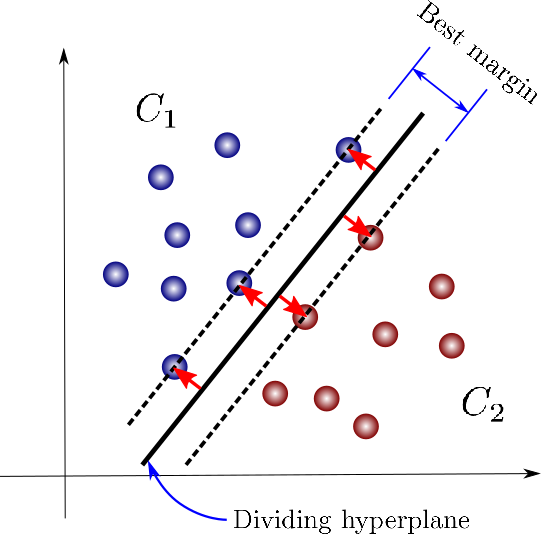
\includegraphics[scale=0.25]{svm.png}\\
	\quelle\url{https://towardsdatascience.com/support-vector-machines-for-classification-fc7c1565e3}
\end{figure}
\end{frame}
%<-------------Folie--------->
\begin{frame}
\frametitle{Analysemethoden}
\framesubtitle{Support Vector Machine}
\begin{itemize}\setlength\parskip{12pt}
	\item Verschiedene Kerne (Funktionen) um dem Separierungsproblem gerecht zu werden
	\item Kerne projizieren nicht-linear separierbare Daten niedrigerer Dimensionen auf linear-separierbare Daten höherer Dimensionen
	\item Vier häufig verwendete Kerne:
	\begin{itemize}
		\item Linear
		\item Polynomiell
		\item Radial
		\item Sigmoidal (Tangens hyperbolicus)
	\end{itemize}
	\item In \texttt{R} mit \texttt{e1071} und in Python mit \texttt{sklearn}
\end{itemize}
\end{frame}
%<-------------Folie--------->
\begin{frame}
\frametitle{Resultate Support Vector Machine, R, mind. 10 mal Wörter, Radialer Kern}
\begin{center}
\begin{tabular}{r|c|c|c|c|}
 &  Dominant  & Gewissenhaft & Initiativ & Stetig\\
\hline
Dominant & 14 & 3 & 8 & 1 \\
Gewissenhaft & 0 & 1 & 1 & 0\\
Initiativ & 4 & 10 & 27 & 14\\
Stetig & 0 & 0 & 0 & 3
\end{tabular}
\end{center}
\end{frame}
%<-------------Folie--------->
\begin{frame}
\frametitle{Resultate Support Vector Machine, R, mind. 10 mal Wörter, Radialer Kern}
\begin{center}
	\begin{tabular}{r|c|c|c|}
		& Precision  & Recall & F1 \\
		\hline
		Dominant     & 53,8\% & 77,8\% & 63,6\% \\
		Gewissenhaft & 50,0\% & 7,1\% & 16,3\% \\
		Initiativ    & 57,0\% & 75,0\% & 41,9\% \\
		Stetig       & 100,0\% & 16,7\% & 20,9\% \\
		\hline
		Macro        & 63,2\% & 44,1\% & 41,0\%
	\end{tabular}
\end{center}
Die Accuracy beträgt ca. 52,33\% und der gewichtete Macro-F1 ca. 46,2\%.
\end{frame}
%<-------------Folie--------->
\begin{frame}
\frametitle{Resultate Support Vector Machine, Python, Englisch, mind. 20 mal Wörter, Sigmoid Kern}
\begin{center}
	\begin{tabular}{r|c|c|c|c|}
		&  Dominant  & Gewissenhaft & Initiativ & Stetig\\
		\hline
		Dominant & 14 & 2 & 9 & 1 \\
		Gewissenhaft & 0 & 5 & 4 & 1\\
		Initiativ & 3 & 5 & 19 & 13\\
		Stetig & 1 & 2 & 4 & 3
	\end{tabular}
\end{center}
\end{frame}
%<-------------Folie--------->
\begin{frame}
\frametitle{Resultate Support Vector Machine, Python, Englisch, mind. 20 mal Wörter, Sigmoid Kern}
\begin{center}
\begin{tabular}{r|c|c|c|}
	& Precision  & Recall & F1 \\
	\hline
	Dominant     & 54\% & 78\% & 64\% \\
	Gewissenhaft & 50\% & 36\% & 42\% \\
	Initiativ    & 47\% & 53\% & 50\% \\
	Stetig       & 30\% & 17\% & 21\% \\
	\hline
	Macro        & 45\% & 46\% & 44\%
\end{tabular}
\end{center}
Die Accuracy beträgt ca. 47,7\% und der gewichtete Macro-F1 ca. 46\%.
\end{frame}
%<-------------Folie--------->
\begin{frame}
\frametitle{Schwierigkeiten}
\begin{itemize}
	\item Keine eindeutige Klassifikation
	\begin{itemize}
		\item Auch für Menschen nicht eindeutig
		\item Teilweise sehr geringe Unterschiede zwischen den Typen
	\end{itemize}
	\item Stemming nicht unbedingt eindeutig
	\begin{itemize}
		\item Unregelmäßigkeit von Verben im Deutschen
		\item Komposita
	\end{itemize}
	\item Geringe Zahl an Trainingsdaten
	\item Unbalanciertes Studiendesign
	\item Representativität
	\begin{itemize}
		\item Introvertierte Kunden schreiben weniger häufig Reviews
		\item Nur positive Bewertungen lagen vor
	\end{itemize}
\end{itemize}
\end{frame}
\end{document}